\clearpage
\section{Auswertung}
	\label{sec:auswertung}
	Im Folgenden werden einige Mittelwerte gebildet.
	Bei einer Anzahl von $n$ Messwerten $x_\mathrm{i}$ gilt f"ur den Mittelwert $x$:
	\begin{equation*}
		x = \frac{1}{n} \sum_{\mathrm{i} = 0}^n {x_\mathrm{i}} \,.
	\end{equation*}

	Die Varianz $\sigma_x$ dieses Wertes, bzw. dessen Fehler $\Delta x$ betragen
	\begin{equation*}
		\Delta x^2 = \sigma_x = \frac{1}{n - 1} \sum_{\mathrm{i} = 0}^n{\left(x_\mathrm{i} - x\right)^2} \,.
	\end{equation*}

	\subsection{Einseitige Einspannung}
	\label{subsec:einseitig}
		Zur Bestimmung des Elastizit"atsmodules der beiden Stangen, wird jeweils eine lineare Ausgleichsrechnung der Form $D(x) = a\chi$ mit Gleichung \eqref{eqn:einseitig} durchgef"uhrt.
		Hierf"ur wird die Durchbiegung $D$ gegen das Argument
		\begin{equation*}
			\chi = Lx^2 - \frac{x^3}{3}
		\end{equation*}

		aufgetragen. Aus der Steigung $a$ l"asst sich mit Kenntnis der Kraft $F$, die am Stab angreift und des Fl"achentr"agheitsmomentes $I$ die Elastizit"at $E$ bestimmen:
		\begin{eqnarray*}
			a & = & \frac{F}{2EI} \\
			\Leftrightarrow \quad E & = & \frac{F}{2aI} \,.
		\end{eqnarray*}

		F"ur die Kraft $F$ gilt mit der Erdbeschleunigung $g = \SI{9.81}{\newton \per \kilo \gram}$:
		\begin{equation*}
			F = mg
		\end{equation*}

		Zun"achst wird ein quadratischer Stab mit Breite $b$ gemessen. Hier gilt f"ur das Fl"achentr"agheitsmoment $I$ und den Fehler $\Delta I$:
		\begin{eqnarray*}
			I & = & \frac{b^4}{12} \,, \\
			\Delta I & = & \frac{b^3}{3}\Delta b \,.
		\end{eqnarray*}

		Der Stab hat eine L"ange von $L = \SI{53}{\centi \meter}$. Die Breite des Stabes wird durch Mittelung "uber zehn Messwerte bestimmt und es folgt:
		\begin{eqnarray*}
			b & = & \SI{9.962(3)}{\milli \meter} \, \\
			\Rightarrow \quad I & = & \SI{820.1(27)}{\milli \meter \tothe{4}} \,. 
		\end{eqnarray*}

		Mit der Gewichtmasse $m$ folgt die Kraft $F$:
		\begin{eqnarray*}
			m & = & \SI{542.5}{\gram} \, \\
			\Rightarrow \quad F & = & \SI{5.322}{\newton} \,.
		\end{eqnarray*}

		Die lineare Ausgleichsrechnung liefert dann:
		\begin{eqnarray*}
			a & = & \SI{4.92(5)e-08}{\milli \meter \tothe{4}} \\
			\Rightarrow \quad E & = & \SI{69.4(8)}{\kilo \newton \per \milli \meter \cubed} \,.
		\end{eqnarray*}

		Anschlie"send wird die Biegung eines zylindrischen Stabes mit Radius $r$ gemessen.
		F"ur das Fl"achentr"agheitsmoment $I$ gilt dabei
		\begin{eqnarray*}
			I & = & \frac{\pi}{4}r^4 \,\\
			\Delta I & = & \pi r^3 \Delta r \,. \\
		\end{eqnarray*}

		Der Radius $r$ wird wiederum durch Mittelung "uber zehn Messwerte des Durchmessers bestimmt und es folgt
		\begin{eqnarray*}
			r & = & \SI{4.972(3)}{\milli \meter} \, \\
			\Rightarrow \quad I & = & \SI{7677(16)}{\milli \meter \tothe{4}} \,. 
		\end{eqnarray*}

		Mit dem Gewicht der Masse $m$ folgt die Kraft $F$:
		\begin{eqnarray*}
			m & = & \SI{267.8}{\gram} \, \\
			\Rightarrow \quad F & = & \SI{2.627}{\newton} \,.
		\end{eqnarray*}

		Die Ausgleichsrechnung liefert hierf"ur:
		\begin{eqnarray*}
			a & = & \SI{3.33(32)e-8}{\milli \meter \tothe{4}} \\
			\Rightarrow \quad E & = & \SI{86.3(7)}{\kilo \newton \per \milli \meter \cubed} \,.
		\end{eqnarray*}

		Tabellen \ref{table:messung1} und \ref{table:ausmasse1} beinhalten die entsprechenden Messdaten.
		Abbildungen \ref{fig:plot1} und \ref{fig:plot2} zeigen die Ausgleichsgerade und die Messwerte.

		\begin{table}[h!]
			\begin{center}
				\caption{Messdaten f"ur Biegung $D$ der St"abe \label{table:messung1}}
				\begin{tabular}{|r|r|r|r|r|r|r|}
					\hline
						\multicolumn{1}{|c|}{} &
						\multicolumn{3}{c|}{Quadratisch} &
						\multicolumn{3}{c|}{Zylindrisch} \\
					\hline
						\multicolumn{1}{|c|}{$x\,[\SI{}{\milli \meter}]$} &  
						\multicolumn{1}{c|}{$D_0\,[\SI{}{\milli \meter}]$} &  
						\multicolumn{1}{c|}{$D_\mathrm{m}\,[\SI{}{\milli \meter}]$} &  
						\multicolumn{1}{c|}{$D\,[\SI{}{\milli \meter}]$} &  
						\multicolumn{1}{c|}{$D_0\,[\SI{}{\milli \meter}]$} &  
						\multicolumn{1}{c|}{$D_\mathrm{m}\,[\SI{}{\milli \meter}]$} &  
						\multicolumn{1}{c|}{$D\,[\SI{}{\milli \meter}]$} \\
					\hline 
					\hline
						\SI{080}{} & \SI{6.61}{} & \SI{2.16}{} & \SI{0.22}{} & \SI{3.17}{} & \SI{0.24}{} & \SI{0.17}{} \\
\SI{110}{} & \SI{6.76}{} & \SI{2.84}{} & \SI{0.36}{} & \SI{3.55}{} & \SI{0.82}{} & \SI{0.27}{} \\
\SI{140}{} & \SI{7.16}{} & \SI{3.57}{} & \SI{0.56}{} & \SI{3.96}{} & \SI{1.48}{} & \SI{0.39}{} \\
\SI{170}{} & \SI{7.52}{} & \SI{4.30}{} & \SI{0.89}{} & \SI{4.40}{} & \SI{2.23}{} & \SI{0.54}{} \\
\SI{200}{} & \SI{7.83}{} & \SI{5.00}{} & \SI{1.02}{} & \SI{4.80}{} & \SI{2.85}{} & \SI{0.69}{} \\
\SI{230}{} & \SI{8.04}{} & \SI{5.51}{} & \SI{1.31}{} & \SI{5.20}{} & \SI{3.48}{} & \SI{0.87}{} \\
\SI{260}{} & \SI{8.10}{} & \SI{5.91}{} & \SI{1.59}{} & \SI{5.55}{} & \SI{4.08}{} & \SI{1.06}{} \\
\SI{290}{} & \SI{8.10}{} & \SI{6.23}{} & \SI{1.87}{} & \SI{5.87}{} & \SI{4.61}{} & \SI{1.26}{} \\
\SI{320}{} & \SI{8.10}{} & \SI{6.51}{} & \SI{2.19}{} & \SI{6.19}{} & \SI{5.13}{} & \SI{1.47}{} \\
\SI{350}{} & \SI{8.07}{} & \SI{6.76}{} & \SI{2.53}{} & \SI{6.48}{} & \SI{5.61}{} & \SI{1.72}{} \\
\SI{380}{} & \SI{8.05}{} & \SI{7.03}{} & \SI{2.83}{} & \SI{6.77}{} & \SI{6.08}{} & \SI{1.95}{} \\
\SI{410}{} & \SI{7.94}{} & \SI{7.05}{} & \SI{3.22}{} & \SI{6.95}{} & \SI{6.41}{} & \SI{2.17}{} \\
\SI{440}{} & \SI{7.84}{} & \SI{7.28}{} & \SI{3.59}{} & \SI{7.13}{} & \SI{6.74}{} & \SI{2.48}{} \\
\SI{470}{} & \SI{7.77}{} & \SI{7.41}{} & \SI{3.92}{} & \SI{7.31}{} & \SI{7.04}{} & \SI{2.73}{} \\
\SI{500}{} & \SI{7.70}{} & \SI{7.48}{} & \SI{4.45}{} & \SI{7.42}{} & \SI{7.25}{} & \SI{2.93}{} \\
					\hline 
				\end{tabular}
			\end{center}
		\end{table}

		\begin{table}[h!]
			\begin{center}
				\caption{Messwerte zur Bestimmung von Breite $b$ und Durchmesser $r$ der St"abe \label{table:ausmasse1}}
				\begin{tabular}{|r|r||r|r|}
					\hline
						\multicolumn{2}{|c|}{$b\,[\SI{}{\milli \meter}]$} & \multicolumn{2}{c|}{$r\,[\SI{}{\milli \meter}]$} \\
					\hline 
					\hline
						\SI{9.968}{} & \SI{9.950}{} & \SI{9.949}{} & \SI{9.945}{} \\
\SI{9.973}{} & \SI{9.959}{} & \SI{9.939}{} & \SI{9.949}{} \\
\SI{9.972}{} & \SI{9.966}{} & \SI{9.936}{} & \SI{9.950}{} \\
\SI{9.965}{} & \SI{9.960}{} & \SI{9.937}{} & \SI{9.944}{} \\
\SI{9.961}{} & \SI{9.949}{} & \SI{9.943}{} & \SI{9.941}{} \\
					\hline 
				\end{tabular}
			\end{center}
		\end{table}

		\begin{figure}[h]
			\centering
			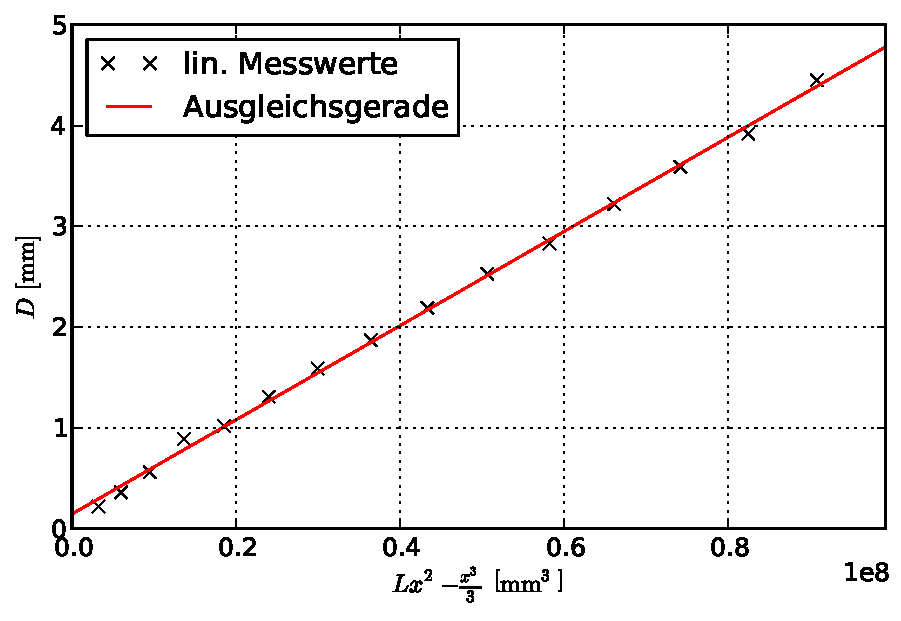
\includegraphics[width = 13cm]{img/plot1.pdf}
			\caption{Lineare Ausgleichsrechnung f"ur den quadratischen Stab \label{fig:plot1}}
		\end{figure}

		\begin{figure}[h]
			\centering
			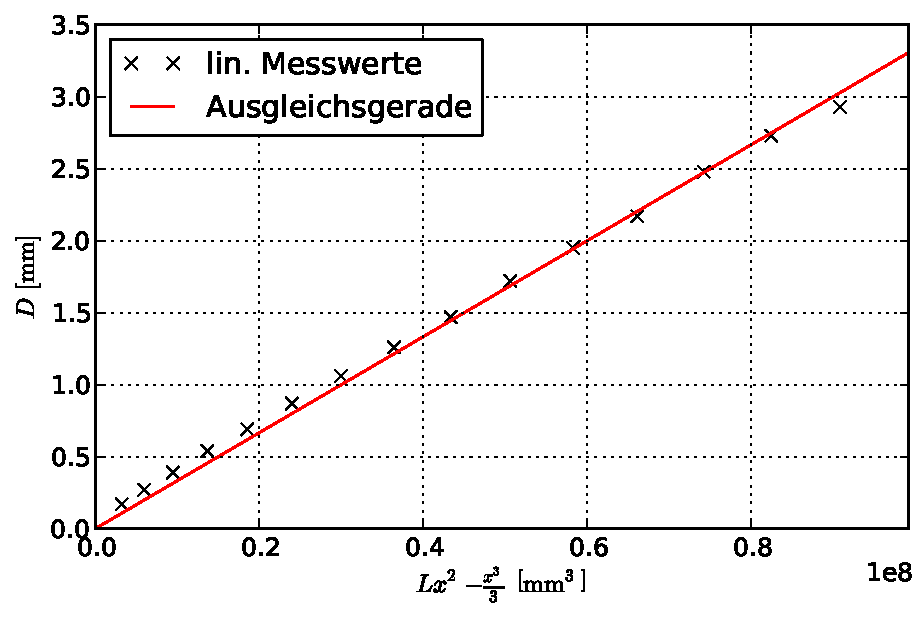
\includegraphics[width = 13cm]{img/plot2.pdf}
			\caption{Lineare Ausgleichsrechnung f"ur den zylindrischen Stab \label{fig:plot2}}
		\end{figure}

		\clearpage

	\subsection{Beidseite Auflage}
	\label{subsec:beidseitig}
		Der zylindrische Stab aus Kapitel \ref{subsec:einseitig} wird nun beidseitig aufgelegt und das Gewicht der Masse $m$ wird mittig befestigt.
		Durch zwei Ausgleichsrechnungen der Form $D = a_\mathrm{re}\chi$ f"ur die rechte Seite des Stabes bzw. $D = a_\mathrm{li}\phi$ f"ur die linke Seite des Stabes lassen sich zwei Werte $E_\mathrm{rechts}$ und $E_\mathrm{links}$ der Elastizit"at bestimmen.

		Dabei ist
		\begin{eqnarray*}
			\chi & = & 3L^2x - 4x^3 \, \\
			\phi & = & 4x^3 - 12 Lx^2 + 9L^2x - L^3 \,, \\
			E_\mathrm{re,li} & = & \frac{F}{48 a_\mathrm{re,li} I} \,.
		\end{eqnarray*}

		Mit dem Gewicht der Masse $m$ folgt die Kraft $F$:
		\begin{eqnarray*}
			m & = & \SI{1648.3}{\gram} \, \\
			\Rightarrow \quad F & = & \SI{16.17}{\newton} \,.
		\end{eqnarray*}

		Das Fl"achentr"agheitsmoment $I$ bleibt unver"andert zu Kapitel \ref{subsec:einseitig}.
		Die L"ange des Stabes betr"agt nun $L = \SI{55.5}{\centi \meter}$.
		Die Ausgleichsrechnungen liefern dann
		\begin{eqnarray*}
			E_\mathrm{re} & = & \SI{81(6)}{\kilo \newton \per \milli \meter \squared} \,, \\
			E_\mathrm{li} & = & \SI{80(1)}{\kilo \newton \per \milli \meter \squared} \,, \\
			\overline{E} = \frac{E_\mathrm{re} + E_\mathrm{li}}{2} & = & \SI{81(6)}{\kilo \newton \per \milli \meter \squared} \,.
		\end{eqnarray*}

		Tabelle \ref{table:messung3} und Abbildung \ref{fig:plot3} zeigen die Messdaten, sowie die Ausgleichsgeraden.

		\begin{table}[h!]
			\begin{center}
				\caption{Messdaten bei beidseitiger Auflage des zylindrischen Stabes \label{table:messung3}}
				\begin{tabular}{|r|r|r|r||r|r|r|r|}
					\hline
						\multicolumn{1}{|c|}{$x\,[\mathrm{mm}]$} & 
						\multicolumn{1}{c|}{$D_0\,[\mathrm{mm}]$} & 
						\multicolumn{1}{c|}{$D_\mathrm{m}\,[\mathrm{mm}]$} &
						\multicolumn{1}{c||}{$D\,[\mathrm{mm}]$} & 
						\multicolumn{1}{c|}{$x\,[\mathrm{mm}]$} & 
						\multicolumn{1}{c|}{$D_0\,[\mathrm{mm}]$} & 
						\multicolumn{1}{c|}{$D_\mathrm{m}\,[\mathrm{mm}]$} &
						\multicolumn{1}{c|}{$D\,[\mathrm{mm}]$} \\
					\hline 
					\hline
						\SI{030}{} & \SI{3.91}{} & \SI{3.54}{} & \SI{0.37}{} & \SI{290}{} & \SI{6.77}{} & \SI{5.05}{} & \SI{1.72}{} \\
\SI{050}{} & \SI{3.85}{} & \SI{3.36}{} & \SI{0.49}{} & \SI{310}{} & \SI{6.80}{} & \SI{5.08}{} & \SI{1.72}{} \\
\SI{070}{} & \SI{3.81}{} & \SI{3.18}{} & \SI{0.63}{} & \SI{330}{} & \SI{6.90}{} & \SI{5.13}{} & \SI{1.77}{} \\
\SI{090}{} & \SI{3.78}{} & \SI{2.99}{} & \SI{0.79}{} & \SI{350}{} & \SI{6.95}{} & \SI{5.20}{} & \SI{1.75}{} \\
\SI{110}{} & \SI{3.73}{} & \SI{2.78}{} & \SI{0.95}{} & \SI{370}{} & \SI{7.00}{} & \SI{5.28}{} & \SI{1.72}{} \\
\SI{130}{} & \SI{3.68}{} & \SI{2.59}{} & \SI{1.09}{} & \SI{390}{} & \SI{7.04}{} & \SI{5.38}{} & \SI{1.66}{} \\
\SI{150}{} & \SI{3.65}{} & \SI{2.43}{} & \SI{1.22}{} & \SI{410}{} & \SI{7.09}{} & \SI{5.52}{} & \SI{1.57}{} \\
\SI{170}{} & \SI{3.60}{} & \SI{2.27}{} & \SI{1.33}{} & \SI{430}{} & \SI{7.14}{} & \SI{5.69}{} & \SI{1.45}{} \\
\SI{190}{} & \SI{3.52}{} & \SI{2.13}{} & \SI{1.39}{} & \SI{450}{} & \SI{7.19}{} & \SI{5.88}{} & \SI{1.31}{} \\
\SI{210}{} & \SI{3.48}{} & \SI{2.00}{} & \SI{1.48}{} & \SI{470}{} & \SI{7.33}{} & \SI{6.21}{} & \SI{1.12}{} \\
\SI{230}{} & \SI{3.45}{} & \SI{1.90}{} & \SI{1.55}{} & \SI{490}{} & \SI{7.45}{} & \SI{6.52}{} & \SI{0.93}{} \\
\SI{250}{} & \SI{3.35}{} & \SI{1.79}{} & \SI{1.56}{} & \SI{510}{} & \SI{7.55}{} & \SI{6.85}{} & \SI{0.70}{} \\
\SI{270}{} & \SI{3.34}{} & \SI{1.77}{} & \SI{1.57}{} & \SI{530}{} & \SI{7.67}{} & \SI{7.23}{} & \SI{0.44}{} \\
					\hline 
				\end{tabular}
			\end{center}
		\end{table}

		\begin{figure}[h]
			\centering
			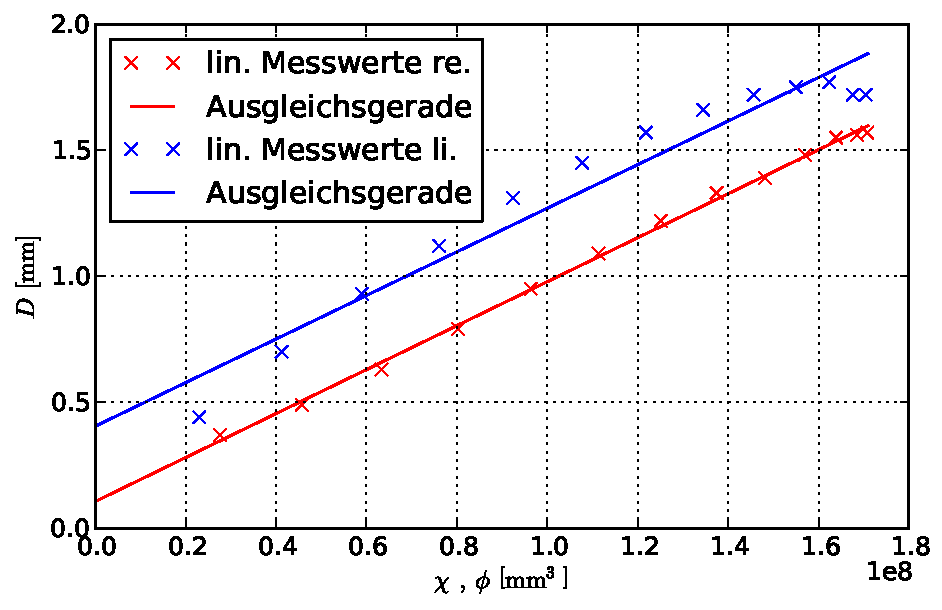
\includegraphics[width = 13cm]{img/plot3.pdf}
			\caption{Ausgleichsgeraden bei beidseitiger Einspannung \label{fig:plot3}}
		\end{figure}

		\clearpage